%% LyX 2.3.3 created this file.  For more info, see http://www.lyx.org/.
%% Do not edit unless you really know what you are doing.
\documentclass[english]{article}
\usepackage[latin1]{inputenc}
\usepackage{geometry}
\geometry{verbose,tmargin=1in,bmargin=1in,lmargin=1in,rmargin=1in,headheight=0in,headsep=0in}
\synctex=-1
\usepackage{color}
\usepackage{babel}
\usepackage{graphicx}
\usepackage{float}
\usepackage[unicode=true]
 {hyperref}

\makeatletter

%%%%%%%%%%%%%%%%%%%%%%%%%%%%%% LyX specific LaTeX commands.
%% Because html converters don't know tabularnewline
\providecommand{\tabularnewline}{\\}

%%%%%%%%%%%%%%%%%%%%%%%%%%%%%% Textclass specific LaTeX commands.
\newenvironment{lyxcode}
	{\par\begin{list}{}{
		\setlength{\rightmargin}{\leftmargin}
		\setlength{\listparindent}{0pt}% needed for AMS classes
		\raggedright
		\setlength{\itemsep}{0pt}
		\setlength{\parsep}{0pt}
		\normalfont\ttfamily}%
	 \item[]}
	{\end{list}}

\makeatother

\begin{document}
\begin{center}
\textbf{\large{}CSCE 221 Cover Page}\\
\bigskip{}
\par\end{center}

First Name~Clayton~~~~~~~~~~~~~~~~~~~~~~~~Last
Name Kristiansen~~~~~~~~~~~~~~~~~~~~~~~UIN~328003173~\bigskip{}

User Name kristiansenc~~~~~~~~~~~~~~~~~~~E-mail
address~kristiansenc@tamu.edu~~\medskip{}

Please list all sources in the table below including web pages which
you used to solve or implement the current homework. If you fail to
cite sources you can get a lower number of points or even zero, read
more on Aggie Honor System Office website: \texttt{\href{http://aggiehonor.tamu.edu/}{http://aggiehonor.tamu.edu/}}\medskip{}
\medskip{}

\noindent \begin{flushleft}
\begin{tabular}{|c|c|c|c|c|}
\hline 
Type of sources  & ~~~~~~~~~~~~~~~~~~~~~~~ & ~~~~~~~~~~~~~~~~~~~~~~~~ & ~~~~~~~~~~~~~~~~~~~~~~~ & ~~~~~~~~~~~~~~~~~~~~~~~\tabularnewline
 &  &  &  & \tabularnewline
\hline 
People & none &  &  & \tabularnewline
 &  &  &  & \tabularnewline
\hline 
Web pages (provide URL)  & none &  &  & \tabularnewline
 &  &  &  & \tabularnewline
\hline 
Printed material & none &  &  & \tabularnewline
 &  &  &  & \tabularnewline
\hline 
Other Sources  & none &  &  & \tabularnewline
 &  &  &  & \tabularnewline
\hline 
\end{tabular}
\par\end{flushleft}

\medskip{}
\medskip{}

\noindent I certify that I have listed all the sources that I used
to develop the solutions/codes to the submitted work.

\noindent \emph{On my honor as an Aggie, I have neither given nor
received any unauthorized help on this academic work}.

\bigskip{}
\bigskip{}

\begin{tabular}{cccccc}
Your Name  & ~Clayton Kristiansen~ &  & ~~~~~~~~~~~~~~~ & Date  & ~03-28-2021~\tabularnewline
\end{tabular}\pagebreak{}

\textbf{Report (20 points)}

Write a brief report and submit it to Canvas. The report should include
the following sections:
\begin{enumerate}
\item A description of the assignment objective, how to compile and run
your program, and an explanation of your program structure (i.e. a
high level description of the functions or classes in your code).

    ~~~~~~~~The objective of this assignment was to create a Binary Search Tree implementation.  
    This implementation was not supposed to be self balancing, but 
    had to include basic insert, search, search cost, and print functionality. The insert 
    function used a recursive method to find the correct place in the tree for inserted
    node. The search function operated in a similar way to the insert function in that it
    recursively searched for a certain value by branching left if the desired value was
    less then the current node, or branching right otherwise. This would continue 
    until either the current node was equal to thedesired value, or the end of a 
    branch was reached. The search cost method simply traveled to each noderecursively 
    and assigned a cost value of 1 plus depth to each node it visited. The inorder print 
    method used an inorder traversal recursive function to print each node in its place 
    in the recursion. Finally, the print level by level method used an interative method and
    a queue to print the tree level by level with emtpy space represented by X.

\item A brief description of the data structure you create (i.e. a theoretical
definition of the data structure and the actual data arrangement in
the classes).

    ~~~~~~~~The data structure in this assignment is a Binary Tree. This means that
    data is organized in a form where each node has two child nodes, who in turn may
    have child nodes of their own, or nullptr in place of actual data. This format 
    means that there is a root node, that branches out into every node.
    The data is inserted into this tree structure such that a nodes left child is
    always less, and its right child is always greater. In this way, data can be searched
    for by comparing the desired value to the current node and recursively continuing
    through the appropriate child. If balanced correctly, this means that a binary tree
    can have an average search time of logn. The Binary Tree structure created in this 
    assignment also kept track of the search costs of each node. Each node 
    kept track of its cost. This value was updated when a node was looked up
    or the Tree was being moved or copied.

\item A description of the implementation of\textcolor{black}{{} (a) individual
search cost and (b) average search cost. Analyze the time complexity
of the functions that (a) calculate the individual search cost and
(b) }sum up the search costs over all the nodes. The recurrences/runtime
functions should be from your functions (insert() for an individual
search cost).

\begin{enumerate}
    \item The insert function has a recurance relation of: 
    \begin{equation}
    T(n) = T(n/2) + O(1)   
    \end{equation}
    This means that, following the general form of this relation, the insert
    function is O(log(n)).
    \item The update search costs function goes to each node and calculates its
    respective search cost to be 1 + its depth. To calculate the average search cost,
    the only extra step would be modify the update search costs function to recursively
    add up the search costs of each node and then divide the total resuly by the number
    of nodes. This process would not change the time complexity of this function which is 
    O(n) because it is required to visit each node exactly once.
\end{enumerate}

\item \textbf{Give an individual search cost in terms of }\textbf{\emph{$n$}}\textbf{
using big-O notation}. Analyze and give the average search costs of
a perfect binary tree and a linear binary tree using big-O notation,
assuming that the following formulas are true (\emph{$n$} denotes
the total number of input data). To be clear, part 3 asks you to analyze
the running time of the functions implemented to compute the individual
and average search cost, while here you must analyze the asymptotic
behavior of the values of the search cost itself (Hint: depth of the
tree affects the individual search cost.)

Formula for perfect binary tree: $\sum_{d=0}^{\log_{2}(n+1)-1}2^{d}(d+1)\simeq(n+1)\cdot\log_{2}(n+1)-n$

Formula for linear binary tree: $\sum_{d=1}^{n}d\simeq n(n+1)/2$

where d represents the depth of the tree.

    ~~~~~~~~The formula for the perfect binary tree clearly shows that, for a tree with
    n elements, the total search cost for every node is:
    \begin{equation}
    (n+1)*log(n+1) - n
    \end{equation}
    ~~~~~~~~To find the average search cost function, the total search cost function must be
    divided by n. The result of this is:
    \begin{equation}
    log(n+1) + log(n+1)/n - 1
    \end{equation}
    ~~~~~~~~Converting this function to its Big-O yields O(log(n)) for perfect binary tree.

    ~~~~~~~~The formula for the linear binary tree clearly shows that, for a tree with
    n elements, the total search cost for every node is:
    \begin{equation}
    n(n+1)/2
    \end{equation}
    ~~~~~~~~To find the average search cost function, the total search cost function must be
    divided by n. The result of this is:
    \begin{equation}
    n/2 + 1/2
    \end{equation}
    ~~~~~~~~Converting this function to its Big-O yields O(n) for linear binary tree.

\item Use BSTree\_main.cpp to run your code to analyze the data files provided.
In case you are unable to compile and run code outside of Mimir, contact
your TA for assistance.
\begin{enumerate}
\item The files \emph{1p}, \emph{2p}, ..., \emph{12p} contain $2^{1}-1$,
$2^{2}-1$,..., and $2^{12}-1$ integers respectively. The integers
make 12 \textbf{perfect binary trees} where all leaves are at the
same depth. Calculate and record the average search cost for each
perfect binary tree. 
\item The files \emph{1r}, \emph{2}r, ..., \emph{12r} contain same number
of integers as above. The integers are randomly ordered and make 12
\textbf{random binary trees}. Calculate and record the average search
cost for each tree. 
\item The files \emph{1l}, \emph{2l}, ..., \emph{12l} contain same number
of integers as above. The integers are in increasing order and make
12 \textbf{linear binary trees}. Calculate and record the average
search cost for each tree. 
\item Include a table and a plot of the average search costs you obtain.
The x axis should be the size of the tree and the y axis should be
the average search cost. In your discussions of experimental results,
compare the curves of search costs with your theoretical analysis
that is derived above.\\

\begin{figure}[H]
    \centering
    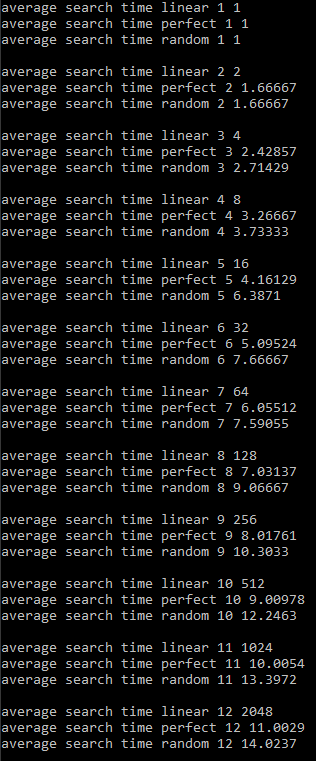
\includegraphics[width=0.6\linewidth]{Records.png}
    \caption{Results}%
    \label{fig:intersection_tests}
 \end{figure}  

 \begin{figure}[H]
    \centering
    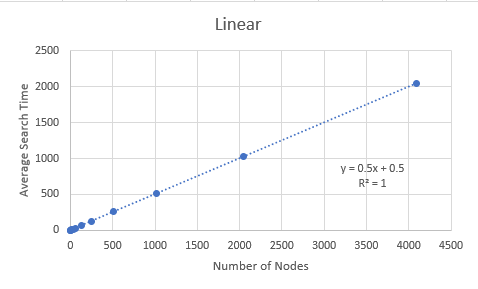
\includegraphics[width=0.8\linewidth]{Linear.png}
    \caption{Linear costs graph}%
    \label{fig:LinearGraph}
 \end{figure}  
 
 \begin{figure}[H]
    \centering
    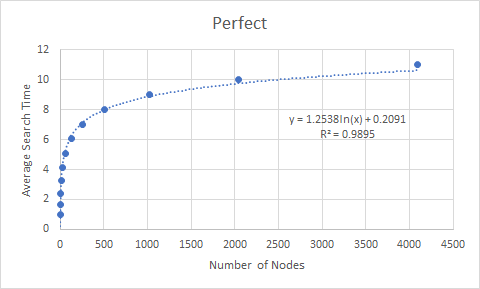
\includegraphics[width=0.8\linewidth]{Perfect.png}
    \caption{Perfect costs graph}%
    \label{fig:PerfectGraph}
 \end{figure}  

 \begin{figure}[H]
    \centering
    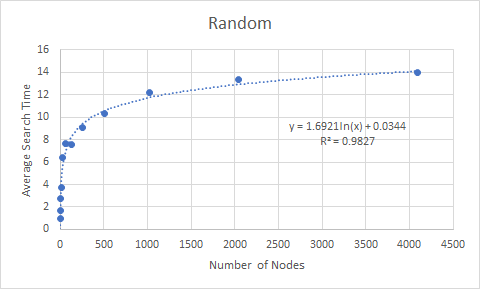
\includegraphics[width=0.8\linewidth]{Random.png}
    \caption{Random costs graph}%
    \label{fig:RandomGraph}
 \end{figure}  

 ~~~~~~~~The theorectical analysis determined that the average search cost for a linear
 Binary Tree should be O(n). This is supported by the data and the graph as it can
 be seen that a linear equation fits the data with an r value of 1.

 ~~~~~~~~The analysis also determined that the average search cost for a perfect
 Binary Tree should be O(log(n)). This is supported by the data and the graph since
 the plot of search costs vs size shows a logarithmic relationship.

 ~~~~~~~~The random Binary Tree also showed a logarithmic average search cost growth 
 function. This makes sense as in previous assignments we have derived the average search
 cost for Binary Trees and they have been O(log(n)). 



\end{enumerate}
\end{enumerate}
\noindent \begin{flushleft}
\texttt{\smallskip{}
}
\par\end{flushleft}
\end{document}
